\chapter{Plating the Triangulars}  

In 1951, D. Alan Stevenson F.R.P.S.L., published his book on Cape Triangulars listing 62 identifiable varieties of the 4d. stamp and suggesting that there was a wide field open for further research. Commander F.W.Collins published an article in the London philatelist in 1960 extending this research. This article draws heavily on both sources.

\section{The Plate Layout}


\ph[width = .98\textwidth]{../cape-of-good-hope/4d-plate.jpg}{Plate Layout as drawn by F.W.Collins.}

\begin{marginfigure}
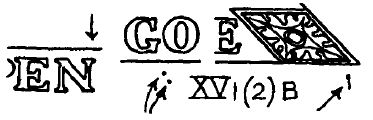
\includegraphics[width = .90\textwidth]{../cape-of-good-hope/4d-identification-example.jpg}
\caption{Most stamps bear individual characteristics, that can enable positioning with the aid of plating guides.}
\end{marginfigure}
\lorem 

\ph[width = .95\textwidth]{../cape-of-good-hope/13027_395_1.jpg}{395  4d. blue with re-entry in 
"POSTAGE", good to large margins, unused with part original
gum; fresh colour and most attractive. S.G. 6a, \pound800. Photo \pound200-250 }    